%%%%%%%%%%%%%%%%%%%%%%%%%%%%%%%%%%%%%%%%%%%%%%%%%%%%%%%%%%%%%%%%%%%%%%%%%%%%%%%%
\begin{frame}{}\label{app_social_science_num}
\Wider[4em]{

\begin{figure}
\input{social_science_area.tex}
\end{figure}
\hyperlink{intro_social_science_ratio}{\beamerbutton{Return: Social science ratio}}
}
\end{frame}

%%%%%%%%%%%%%%%%%%%%%%%%%%%%%%%%%%%%%%%%%%%%%%%%%%%%%%%%%%%%%%%%%%%%%%%%%%%%%%%%
\begin{frame}{Social Sciences}\label{app_social_science_cip}
\Wider[4em]{

\begin{figure}
\setlength{\abovecaptionskip}{2pt}
\setlength{\belowcaptionskip}{-2pt}
\input{cip45.tex}
\end{figure}
\hyperlink{intro_social_science_ratio}{\beamerbutton{Return: Social science ratio}}
}
\end{frame}

%%%%%%%%%%%%%%%%%%%%%%%%%%%%%%%%%%%%%%%%%%%%%%%%%%%%%%%%%%%%%%%%%%%%%%%%%%%%%%%%
\begin{frame}{Engineering}\label{app_engineering}
\Wider[4em]{

\begin{figure}
\setlength{\abovecaptionskip}{2pt}
\setlength{\belowcaptionskip}{-2pt}
\input{cip14.tex}
\end{figure}
\hyperlink{intro_social_science_ratio}{\beamerbutton{Return: Social science ratio}}
}
\end{frame}

%%%%%%%%%%%%%%%%%%%%%%%%%%%%%%%%%%%%%%%%%%%%%%%%%%%%%%%%%%%%%%%%%%%%%%%%%%%%%%%%
\begin{frame}{Business}\label{app_business}
\Wider[4em]{

\begin{figure}
\setlength{\abovecaptionskip}{2pt}
\setlength{\belowcaptionskip}{-2pt}
\input{cip52.tex}
\end{figure}
\hyperlink{intro_social_science_ratio}{\beamerbutton{Return: Social science ratio}}
}
\end{frame}

%%%%%%%%%%%%%%%%%%%%%%%%%%%%%%%%%%%%%%%%%%%%%%%%%%%%%%%%%%%%%%%%%%%%%%%%%%%%%%%%
\begin{frame}{Computer Science}\label{app_computer_science}
\Wider[4em]{

\begin{figure}
\setlength{\abovecaptionskip}{2pt}
\setlength{\belowcaptionskip}{-2pt}
% This file was created by tikzplotlib v0.9.2.
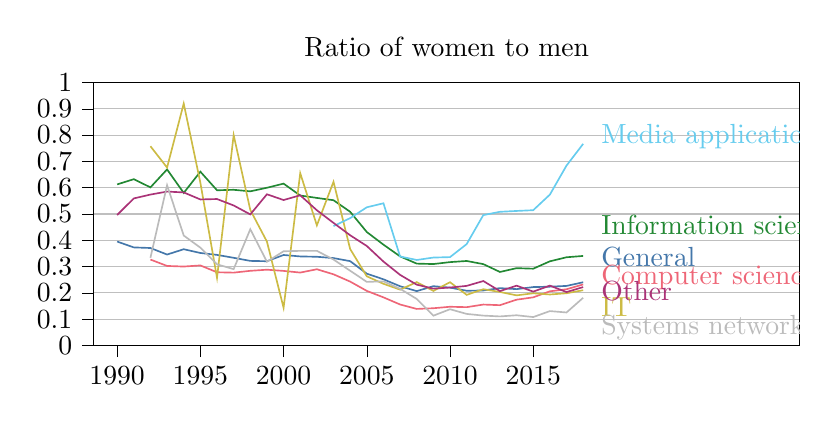
\begin{tikzpicture}

\definecolor{color0}{rgb}{0.266666666666667,0.466666666666667,0.666666666666667}
\definecolor{color1}{rgb}{0.933333333333333,0.4,0.466666666666667}
\definecolor{color2}{rgb}{0.133333333333333,0.533333333333333,0.2}
\definecolor{color3}{rgb}{0.8,0.733333333333333,0.266666666666667}
\definecolor{color4}{rgb}{0.4,0.8,0.933333333333333}
\definecolor{color5}{rgb}{0.666666666666667,0.2,0.466666666666667}

\begin{axis}[
height=140pt,
tick align=outside,
tick pos=left,
title={Ratio of women to men},
unbounded coords=jump,
width=300pt,
x grid style={white!69.0196078431373!black},
xmin=1988.6, xmax=2031,
xtick style={color=black},
xtick={1990,1995,2000,2005,2010,2015},
xticklabels={\(\displaystyle 1990\),\(\displaystyle 1995\),\(\displaystyle 2000\),\(\displaystyle 2005\),\(\displaystyle 2010\),\(\displaystyle 2015\)},
ymajorgrids,
ymin=0, ymax=1,
ytick style={color=black},
ytick={0,0.1,0.2,0.3,0.4,0.5,0.6,0.7,0.8,0.9,1},
yticklabels={\(\displaystyle 0\),\(\displaystyle 0.1\),\(\displaystyle 0.2\),\(\displaystyle 0.3\),\(\displaystyle 0.4\),\(\displaystyle 0.5\),\(\displaystyle 0.6\),\(\displaystyle 0.7\),\(\displaystyle 0.8\),\(\displaystyle 0.9\),\(\displaystyle 1\)}
]
\addplot [semithick, color0]
table {%
1990 0.394967913627625
1991 0.37271773815155
1992 0.370465278625488
1993 0.345574140548706
1994 0.365840792655945
1995 0.351528167724609
1996 0.344272255897522
1997 0.3332200050354
1998 0.321436882019043
1999 0.320170640945435
2000 0.343914747238159
2001 0.338396310806274
2002 0.337104439735413
2003 0.332112669944763
2004 0.320477366447449
2005 0.272923469543457
2006 0.251452445983887
2007 0.225056648254395
2008 0.206436157226562
2009 0.225293636322021
2010 0.219744563102722
2011 0.207880258560181
2012 0.208938837051392
2013 0.217817306518555
2014 0.214048385620117
2015 0.221825838088989
2016 0.223389029502869
2017 0.226261734962463
2018 0.240228176116943
};
\addplot [semithick, color1]
table {%
1990 nan
1991 nan
1992 0.3265465935787
1993 0.302248126561199
1994 0.2999222999223
1995 0.304198473282443
1996 0.278148148148148
1997 0.276795380728979
1998 0.283663704716336
1999 0.287935502447452
2000 0.283360408447436
2001 0.276973281664287
2002 0.289675114815445
2003 0.270382165605096
2004 0.242696416753333
2005 0.207340962985875
2006 0.182779629842511
2007 0.155608214849921
2008 0.13874859708193
2009 0.14136500214623
2010 0.146981988175443
2011 0.145420088439671
2012 0.155357142857143
2013 0.15297619047619
2014 0.173902111967818
2015 0.1828334168516
2016 0.205791482401405
2017 0.2134888957118
2018 0.231927175843694
};
\addplot [semithick, color2]
table {%
1990 0.612352168199737
1991 0.632269348491474
1992 0.601075750784402
1993 0.669402644778842
1994 0.580039920159681
1995 0.66078753076292
1996 0.590057361376673
1997 0.591881116346502
1998 0.586007702182285
1999 0.599660729431722
2000 0.615333035315154
2001 0.570116566584246
2002 0.560919540229885
2003 0.552210724365005
2004 0.508236165093467
2005 0.431290064102564
2006 0.383183709218305
2007 0.338664635694339
2008 0.311026615969582
2009 0.309437854564208
2010 0.316780821917808
2011 0.321109328443731
2012 0.309195912927588
2013 0.279330792037272
2014 0.293806030969845
2015 0.291763791763792
2016 0.319848771266541
2017 0.335242527295507
2018 0.340254305488492
};
\addplot [semithick, color3]
table {%
1990 nan
1991 nan
1992 0.757575757575758
1993 0.676470588235294
1994 0.92
1995 0.619047619047619
1996 0.257142857142857
1997 0.8
1998 0.515151515151515
1999 0.394736842105263
2000 0.142857142857143
2001 0.655172413793103
2002 0.456521739130435
2003 0.622327790973872
2004 0.366598778004073
2005 0.26284751474305
2006 0.234259259259259
2007 0.212081418253447
2008 0.240674501788452
2009 0.20728441349759
2010 0.24040404040404
2011 0.192297111416781
2012 0.213741987179487
2013 0.203204661325564
2014 0.190322580645161
2015 0.198224852071006
2016 0.193636363636364
2017 0.198331193838254
2018 0.209817893903405
};
\addplot [semithick, color4]
table {%
1990 nan
1991 nan
1992 nan
1993 nan
1994 nan
1995 nan
1996 nan
1997 nan
1998 nan
1999 nan
2000 nan
2001 nan
2002 nan
2003 0.453731343283582
2004 0.48406862745098
2005 0.52530779753762
2006 0.540609137055838
2007 0.338213762811127
2008 0.324987963408763
2009 0.334102445777573
2010 0.335807050092764
2011 0.385281385281385
2012 0.495648734177215
2013 0.508133230054222
2014 0.511384845091452
2015 0.514325974635979
2016 0.573572120038722
2017 0.684032802701399
2018 0.766576819407008
};
\addplot [semithick, color5]
table {%
1990 0.496227510156703
1991 0.559025133282559
1992 0.573730862207897
1993 0.585096596136155
1994 0.581833761782348
1995 0.555163283318623
1996 0.556741028128031
1997 0.532289628180039
1998 0.498251748251748
1999 0.57484076433121
2000 0.55296343001261
2001 0.571029529130088
2002 0.514033427940713
2003 0.465948777648428
2004 0.418907007492287
2005 0.37811320754717
2006 0.318900343642612
2007 0.268292682926829
2008 0.230987246102976
2009 0.21584440227704
2010 0.220114689016321
2011 0.226400613967767
2012 0.244788164088769
2013 0.206656101426307
2014 0.227162209100382
2015 0.204568700988749
2016 0.227431770468859
2017 0.202842873607376
2018 0.221844453888653
};
\addplot [semithick, white!73.3333333333333!black]
table {%
1990 nan
1991 nan
1992 0.333333333333333
1993 0.609375
1994 0.417910447761194
1995 0.371794871794872
1996 0.308411214953271
1997 0.290123456790123
1998 0.441913439635535
1999 0.318181818181818
2000 0.358090185676393
2001 0.359615384615385
2002 0.35969387755102
2003 0.326538931920098
2004 0.284086112283664
2005 0.241577335375191
2006 0.243598862019915
2007 0.215324927255092
2008 0.176638176638177
2009 0.113035551504102
2010 0.137533274179237
2011 0.119799139167862
2012 0.113329040566645
2013 0.110236220472441
2014 0.114686951433587
2015 0.107761027359017
2016 0.130511463844797
2017 0.125265392781316
2018 0.181153533712429
};
\draw (axis cs:2018.5,0.300228192859772) node[
  anchor=base west,
  text=color0,
  rotate=0.0
]{General};
\draw (axis cs:2018.5,0.231927175843694) node[
  anchor=base west,
  text=color1,
  rotate=0.0
]{Computer science};
\draw (axis cs:2018.5,0.420254305488492) node[
  anchor=base west,
  text=color2,
  rotate=0.0
]{Information science};
\draw (axis cs:2018.5,0.109817893903405) node[
  anchor=base west,
  text=color3,
  rotate=0.0
]{IT};
\draw (axis cs:2018.5,0.766576819407008) node[
  anchor=base west,
  text=color4,
  rotate=0.0
]{Media applications};
\draw (axis cs:2018.5,0.171844453888653) node[
  anchor=base west,
  text=color5,
  rotate=0.0
]{Other};
\draw (axis cs:2018.5,0.0411535337124289) node[
  anchor=base west,
  text=white!73.3333333333333!black,
  rotate=0.0
]{Systems network};
\end{axis}

\end{tikzpicture}

\vspace{0.1cm}
\begin{tikzpicture}
% This file was created by tikzplotlib v0.9.2.
\definecolor{color0}{rgb}{0.266666666666667,0.466666666666667,0.666666666666667}
\definecolor{color1}{rgb}{0.933333333333333,0.4,0.466666666666667}
\definecolor{color2}{rgb}{0.133333333333333,0.533333333333333,0.2}
\definecolor{color3}{rgb}{0.8,0.733333333333333,0.266666666666667}
\definecolor{color4}{rgb}{0.4,0.8,0.933333333333333}
\definecolor{color5}{rgb}{0.666666666666667,0.2,0.466666666666667}

\begin{groupplot}[group style={group size=2 by 1, group name=my plots, horizontal sep=0.8cm}]
\nextgroupplot[
height=90pt, width=160pt,
legend style={at={(2.02, 0.5)},anchor=west,},
reverse legend,
tick align=outside,
tick pos=left,
x grid style={white!69.0196078431373!black},
xlabel={Women},
xmin=1988.6, xmax=2019.4,
xtick style={color=black},
xtick={1990,2000,2010},
xticklabels={\(\displaystyle 1990\),\(\displaystyle 2000\),\(\displaystyle 2010\)},
ymajorgrids,
ymin=0, ymax=17.94555,
ytick style={color=black}
]
\path [draw=color0, fill=color0]
(axis cs:1990,6.028)
--(axis cs:1990,0)
--(axis cs:1991,0)
--(axis cs:1992,0)
--(axis cs:1993,0)
--(axis cs:1994,0)
--(axis cs:1995,0)
--(axis cs:1996,0)
--(axis cs:1997,0)
--(axis cs:1998,0)
--(axis cs:1999,0)
--(axis cs:2000,0)
--(axis cs:2001,0)
--(axis cs:2002,0)
--(axis cs:2003,0)
--(axis cs:2004,0)
--(axis cs:2005,0)
--(axis cs:2006,0)
--(axis cs:2007,0)
--(axis cs:2008,0)
--(axis cs:2009,0)
--(axis cs:2010,0)
--(axis cs:2011,0)
--(axis cs:2012,0)
--(axis cs:2013,0)
--(axis cs:2014,0)
--(axis cs:2015,0)
--(axis cs:2016,0)
--(axis cs:2017,0)
--(axis cs:2018,0)
--(axis cs:2018,6.527)
--(axis cs:2018,6.527)
--(axis cs:2017,5.483)
--(axis cs:2016,4.85)
--(axis cs:2015,4.291)
--(axis cs:2014,3.736)
--(axis cs:2013,3.423)
--(axis cs:2012,3.048)
--(axis cs:2011,2.944)
--(axis cs:2010,2.976)
--(axis cs:2009,3.203)
--(axis cs:2008,2.489)
--(axis cs:2007,3.679)
--(axis cs:2006,4.501)
--(axis cs:2005,5.566)
--(axis cs:2004,6.955)
--(axis cs:2003,6.439)
--(axis cs:2002,6.913)
--(axis cs:2001,6.461)
--(axis cs:2000,5.612)
--(axis cs:1999,4.354)
--(axis cs:1998,4.152)
--(axis cs:1997,3.922)
--(axis cs:1996,3.955)
--(axis cs:1995,4.083)
--(axis cs:1994,4.164)
--(axis cs:1993,4.15)
--(axis cs:1992,4.34)
--(axis cs:1991,5.328)
--(axis cs:1990,6.028)
--cycle;

\path [draw=color1, fill=color1]
(axis cs:1990,6.028)
--(axis cs:1990,6.028)
--(axis cs:1991,5.328)
--(axis cs:1992,4.34)
--(axis cs:1993,4.15)
--(axis cs:1994,4.164)
--(axis cs:1995,4.083)
--(axis cs:1996,3.955)
--(axis cs:1997,3.922)
--(axis cs:1998,4.152)
--(axis cs:1999,4.354)
--(axis cs:2000,5.612)
--(axis cs:2001,6.461)
--(axis cs:2002,6.913)
--(axis cs:2003,6.439)
--(axis cs:2004,6.955)
--(axis cs:2005,5.566)
--(axis cs:2006,4.501)
--(axis cs:2007,3.679)
--(axis cs:2008,2.489)
--(axis cs:2009,3.203)
--(axis cs:2010,2.976)
--(axis cs:2011,2.944)
--(axis cs:2012,3.048)
--(axis cs:2013,3.423)
--(axis cs:2014,3.736)
--(axis cs:2015,4.291)
--(axis cs:2016,4.85)
--(axis cs:2017,5.483)
--(axis cs:2018,6.527)
--(axis cs:2018,11.75)
--(axis cs:2018,11.75)
--(axis cs:2017,9.655)
--(axis cs:2016,8.247)
--(axis cs:2015,6.845)
--(axis cs:2014,5.811)
--(axis cs:2013,4.965)
--(axis cs:2012,4.44)
--(axis cs:2011,4.095)
--(axis cs:2010,4.045)
--(axis cs:2009,4.191)
--(axis cs:2008,3.478)
--(axis cs:2007,4.861)
--(axis cs:2006,6.091)
--(axis cs:2005,7.577)
--(axis cs:2004,9.522)
--(axis cs:2003,8.986)
--(axis cs:2002,8.616)
--(axis cs:2001,7.819)
--(axis cs:2000,6.833)
--(axis cs:1999,5.354)
--(axis cs:1998,4.982)
--(axis cs:1997,4.689)
--(axis cs:1996,4.706)
--(axis cs:1995,4.88)
--(axis cs:1994,4.936)
--(axis cs:1993,4.876)
--(axis cs:1992,5.174)
--(axis cs:1991,5.328)
--(axis cs:1990,6.028)
--cycle;

\path [draw=color2, fill=color2]
(axis cs:1990,7.426)
--(axis cs:1990,6.028)
--(axis cs:1991,5.328)
--(axis cs:1992,5.174)
--(axis cs:1993,4.876)
--(axis cs:1994,4.936)
--(axis cs:1995,4.88)
--(axis cs:1996,4.706)
--(axis cs:1997,4.689)
--(axis cs:1998,4.982)
--(axis cs:1999,5.354)
--(axis cs:2000,6.833)
--(axis cs:2001,7.819)
--(axis cs:2002,8.616)
--(axis cs:2003,8.986)
--(axis cs:2004,9.522)
--(axis cs:2005,7.577)
--(axis cs:2006,6.091)
--(axis cs:2007,4.861)
--(axis cs:2008,3.478)
--(axis cs:2009,4.191)
--(axis cs:2010,4.045)
--(axis cs:2011,4.095)
--(axis cs:2012,4.44)
--(axis cs:2013,4.965)
--(axis cs:2014,5.811)
--(axis cs:2015,6.845)
--(axis cs:2016,8.247)
--(axis cs:2017,9.655)
--(axis cs:2018,11.75)
--(axis cs:2018,13.864)
--(axis cs:2018,13.864)
--(axis cs:2017,11.528)
--(axis cs:2016,9.939)
--(axis cs:2015,8.347)
--(axis cs:2014,7.253)
--(axis cs:2013,6.284)
--(axis cs:2012,5.832)
--(axis cs:2011,5.496)
--(axis cs:2010,5.34)
--(axis cs:2009,5.391)
--(axis cs:2008,4.705)
--(axis cs:2007,6.195)
--(axis cs:2006,7.841)
--(axis cs:2005,9.73)
--(axis cs:2004,12.268)
--(axis cs:2003,13.095)
--(axis cs:2002,12.276)
--(axis cs:2001,11.047)
--(axis cs:2000,9.586)
--(axis cs:1999,7.475)
--(axis cs:1998,6.808)
--(axis cs:1997,6.322)
--(axis cs:1996,6.249)
--(axis cs:1995,6.491)
--(axis cs:1994,6.389)
--(axis cs:1993,6.344)
--(axis cs:1992,6.515)
--(axis cs:1991,6.774)
--(axis cs:1990,7.426)
--cycle;

\path [draw=color3, fill=color3]
(axis cs:1990,7.426)
--(axis cs:1990,7.426)
--(axis cs:1991,6.774)
--(axis cs:1992,6.515)
--(axis cs:1993,6.344)
--(axis cs:1994,6.389)
--(axis cs:1995,6.491)
--(axis cs:1996,6.249)
--(axis cs:1997,6.322)
--(axis cs:1998,6.808)
--(axis cs:1999,7.475)
--(axis cs:2000,9.586)
--(axis cs:2001,11.047)
--(axis cs:2002,12.276)
--(axis cs:2003,13.095)
--(axis cs:2004,12.268)
--(axis cs:2005,9.73)
--(axis cs:2006,7.841)
--(axis cs:2007,6.195)
--(axis cs:2008,4.705)
--(axis cs:2009,5.391)
--(axis cs:2010,5.34)
--(axis cs:2011,5.496)
--(axis cs:2012,5.832)
--(axis cs:2013,6.284)
--(axis cs:2014,7.253)
--(axis cs:2015,8.347)
--(axis cs:2016,9.939)
--(axis cs:2017,11.528)
--(axis cs:2018,13.864)
--(axis cs:2018,14.924)
--(axis cs:2018,14.924)
--(axis cs:2017,12.455)
--(axis cs:2016,10.791)
--(axis cs:2015,9.419)
--(axis cs:2014,8.315)
--(axis cs:2013,7.4)
--(axis cs:2012,6.899)
--(axis cs:2011,6.195)
--(axis cs:2010,5.935)
--(axis cs:2009,5.778)
--(axis cs:2008,5.647)
--(axis cs:2007,6.518)
--(axis cs:2006,8.094)
--(axis cs:2005,10.042)
--(axis cs:2004,12.448)
--(axis cs:2003,13.357)
--(axis cs:2002,12.297)
--(axis cs:2001,11.066)
--(axis cs:2000,9.591)
--(axis cs:1999,7.49)
--(axis cs:1998,6.825)
--(axis cs:1997,6.338)
--(axis cs:1996,6.258)
--(axis cs:1995,6.504)
--(axis cs:1994,6.412)
--(axis cs:1993,6.367)
--(axis cs:1992,6.54)
--(axis cs:1991,6.774)
--(axis cs:1990,7.426)
--cycle;

\path [draw=color4, fill=color4]
(axis cs:1990,7.426)
--(axis cs:1990,7.426)
--(axis cs:1991,6.774)
--(axis cs:1992,6.54)
--(axis cs:1993,6.367)
--(axis cs:1994,6.412)
--(axis cs:1995,6.504)
--(axis cs:1996,6.258)
--(axis cs:1997,6.338)
--(axis cs:1998,6.825)
--(axis cs:1999,7.49)
--(axis cs:2000,9.591)
--(axis cs:2001,11.066)
--(axis cs:2002,12.297)
--(axis cs:2003,13.357)
--(axis cs:2004,12.448)
--(axis cs:2005,10.042)
--(axis cs:2006,8.094)
--(axis cs:2007,6.518)
--(axis cs:2008,5.647)
--(axis cs:2009,5.778)
--(axis cs:2010,5.935)
--(axis cs:2011,6.195)
--(axis cs:2012,6.899)
--(axis cs:2013,7.4)
--(axis cs:2014,8.315)
--(axis cs:2015,9.419)
--(axis cs:2016,10.791)
--(axis cs:2017,12.455)
--(axis cs:2018,14.924)
--(axis cs:2018,16.346)
--(axis cs:2018,16.346)
--(axis cs:2017,13.873)
--(axis cs:2016,11.976)
--(axis cs:2015,10.514)
--(axis cs:2014,9.685)
--(axis cs:2013,8.712)
--(axis cs:2012,8.152)
--(axis cs:2011,7.174)
--(axis cs:2010,6.84)
--(axis cs:2009,6.502)
--(axis cs:2008,6.322)
--(axis cs:2007,6.98)
--(axis cs:2006,8.52)
--(axis cs:2005,10.426)
--(axis cs:2004,12.843)
--(axis cs:2003,13.661)
--(axis cs:2002,12.297)
--(axis cs:2001,11.066)
--(axis cs:2000,9.591)
--(axis cs:1999,7.49)
--(axis cs:1998,6.825)
--(axis cs:1997,6.338)
--(axis cs:1996,6.258)
--(axis cs:1995,6.504)
--(axis cs:1994,6.412)
--(axis cs:1993,6.367)
--(axis cs:1992,6.54)
--(axis cs:1991,6.774)
--(axis cs:1990,7.426)
--cycle;

\path [draw=color5, fill=color5]
(axis cs:1990,8.281)
--(axis cs:1990,7.426)
--(axis cs:1991,6.774)
--(axis cs:1992,6.54)
--(axis cs:1993,6.367)
--(axis cs:1994,6.412)
--(axis cs:1995,6.504)
--(axis cs:1996,6.258)
--(axis cs:1997,6.338)
--(axis cs:1998,6.825)
--(axis cs:1999,7.49)
--(axis cs:2000,9.591)
--(axis cs:2001,11.066)
--(axis cs:2002,12.297)
--(axis cs:2003,13.661)
--(axis cs:2004,12.843)
--(axis cs:2005,10.426)
--(axis cs:2006,8.52)
--(axis cs:2007,6.98)
--(axis cs:2008,6.322)
--(axis cs:2009,6.502)
--(axis cs:2010,6.84)
--(axis cs:2011,7.174)
--(axis cs:2012,8.152)
--(axis cs:2013,8.712)
--(axis cs:2014,9.685)
--(axis cs:2015,10.514)
--(axis cs:2016,11.976)
--(axis cs:2017,13.873)
--(axis cs:2018,16.346)
--(axis cs:2018,16.868)
--(axis cs:2018,16.868)
--(axis cs:2017,14.401)
--(axis cs:2016,12.626)
--(axis cs:2015,11.114)
--(axis cs:2014,10.339)
--(axis cs:2013,9.364)
--(axis cs:2012,8.88)
--(axis cs:2011,7.764)
--(axis cs:2010,7.339)
--(axis cs:2009,6.957)
--(axis cs:2008,6.811)
--(axis cs:2007,7.651)
--(axis cs:2006,9.448)
--(axis cs:2005,11.929)
--(axis cs:2004,14.744)
--(axis cs:2003,15.262)
--(axis cs:2002,13.927)
--(axis cs:2001,12.497)
--(axis cs:2000,10.468)
--(axis cs:1999,8.212)
--(axis cs:1998,7.395)
--(axis cs:1997,6.882)
--(axis cs:1996,6.832)
--(axis cs:1995,7.133)
--(axis cs:1994,7.091)
--(axis cs:1993,7.003)
--(axis cs:1992,7.252)
--(axis cs:1991,7.508)
--(axis cs:1990,8.281)
--cycle;

\path [draw=white!73.3333333333333!black, fill=white!73.3333333333333!black]
(axis cs:1990,8.281)
--(axis cs:1990,8.281)
--(axis cs:1991,7.508)
--(axis cs:1992,7.252)
--(axis cs:1993,7.003)
--(axis cs:1994,7.091)
--(axis cs:1995,7.133)
--(axis cs:1996,6.832)
--(axis cs:1997,6.882)
--(axis cs:1998,7.395)
--(axis cs:1999,8.212)
--(axis cs:2000,10.468)
--(axis cs:2001,12.497)
--(axis cs:2002,13.927)
--(axis cs:2003,15.262)
--(axis cs:2004,14.744)
--(axis cs:2005,11.929)
--(axis cs:2006,9.448)
--(axis cs:2007,7.651)
--(axis cs:2008,6.811)
--(axis cs:2009,6.957)
--(axis cs:2010,7.339)
--(axis cs:2011,7.764)
--(axis cs:2012,8.88)
--(axis cs:2013,9.364)
--(axis cs:2014,10.339)
--(axis cs:2015,11.114)
--(axis cs:2016,12.626)
--(axis cs:2017,14.401)
--(axis cs:2018,16.868)
--(axis cs:2018,17.091)
--(axis cs:2018,17.091)
--(axis cs:2017,14.578)
--(axis cs:2016,12.848)
--(axis cs:2015,11.307)
--(axis cs:2014,10.535)
--(axis cs:2013,9.546)
--(axis cs:2012,9.056)
--(axis cs:2011,7.931)
--(axis cs:2010,7.494)
--(axis cs:2009,7.081)
--(axis cs:2008,7.059)
--(axis cs:2007,8.095)
--(axis cs:2006,10.133)
--(axis cs:2005,12.56)
--(axis cs:2004,15.417)
--(axis cs:2003,16.063)
--(axis cs:2002,14.491)
--(axis cs:2001,12.871)
--(axis cs:2000,10.738)
--(axis cs:1999,8.408)
--(axis cs:1998,7.589)
--(axis cs:1997,6.976)
--(axis cs:1996,6.865)
--(axis cs:1995,7.162)
--(axis cs:1994,7.119)
--(axis cs:1993,7.042)
--(axis cs:1992,7.278)
--(axis cs:1991,7.508)
--(axis cs:1990,8.281)
--cycle;

\addplot [semithick, color0]
table {%
1990 6.02799987792969
1991 5.32800006866455
1992 4.34000015258789
1993 4.15000009536743
1994 4.16400003433228
1995 4.08300018310547
1996 3.95499992370605
1997 3.92199993133545
1998 4.15199995040894
1999 4.35400009155273
2000 5.61199998855591
2001 6.46099996566772
2002 6.91300010681152
2003 6.43900012969971
2004 6.95499992370605
2005 5.56599998474121
2006 4.50099992752075
2007 3.67899990081787
2008 2.48900008201599
2009 3.20300006866455
2010 2.9760000705719
2011 2.94400000572205
2012 3.04800009727478
2013 3.42300009727478
2014 3.73600006103516
2016 4.84999990463257
2017 5.48299980163574
2018 6.52699995040894
};
\addplot [semithick, color1]
table {%
1990 6.02799987792969
1991 5.32800006866455
1992 5.17399978637695
1993 4.87599992752075
1994 4.93599987030029
1995 4.88000011444092
1996 4.70599985122681
1997 4.68900012969971
1998 4.98199987411499
1999 5.35400009155273
2000 6.83300018310547
2001 7.81899976730347
2002 8.61600017547607
2003 8.98600006103516
2004 9.52200031280518
2005 7.5770001411438
2006 6.09100008010864
2007 4.86100006103516
2008 3.4779999256134
2009 4.19099998474121
2010 4.04500007629395
2011 4.09499979019165
2012 4.44000005722046
2013 4.96500015258789
2014 5.81099987030029
2015 6.84499979019165
2017 9.65499973297119
2018 11.75
};
\addplot [semithick, color2]
table {%
1990 7.42600011825562
1991 6.77400016784668
1992 6.5149998664856
1993 6.3439998626709
1994 6.38899993896484
1995 6.49100017547607
1996 6.24900007247925
1997 6.32200002670288
1998 6.80800008773804
1999 7.47499990463257
2000 9.58600044250488
2001 11.0469999313354
2002 12.2760000228882
2003 13.0950002670288
2004 12.2679996490479
2005 9.72999954223633
2006 7.84100008010864
2007 6.19500017166138
2008 4.70499992370605
2009 5.39099979400635
2010 5.34000015258789
2011 5.49599981307983
2012 5.83199977874756
2013 6.28399991989136
2014 7.25299978256226
2015 8.34700012207031
2017 11.5279998779297
2018 13.8640003204346
};
\addplot [semithick, color3]
table {%
1990 7.42600011825562
1991 6.77400016784668
1992 6.53999996185303
1993 6.36700010299683
1994 6.41200017929077
1995 6.50400018692017
1996 6.25799989700317
1997 6.33799982070923
1998 6.82499980926514
1999 7.48999977111816
2000 9.59099960327148
2001 11.0659999847412
2002 12.2969999313354
2003 13.3570003509521
2004 12.4479999542236
2005 10.0419998168945
2006 8.0939998626709
2007 6.51800012588501
2008 5.64699983596802
2009 5.77799987792969
2010 5.93499994277954
2011 6.19500017166138
2012 6.89900016784668
2013 7.40000009536743
2014 8.3149995803833
2015 9.41899967193604
2016 10.7910003662109
2017 12.4549999237061
2018 14.923999786377
};
\addplot [semithick, color4]
table {%
1990 7.42600011825562
1991 6.77400016784668
1992 6.53999996185303
1993 6.36700010299683
1994 6.41200017929077
1995 6.50400018692017
1996 6.25799989700317
1997 6.33799982070923
1998 6.82499980926514
1999 7.48999977111816
2000 9.59099960327148
2001 11.0659999847412
2002 12.2969999313354
2003 13.66100025177
2004 12.8430004119873
2005 10.4259996414185
2006 8.52000045776367
2007 6.98000001907349
2008 6.32200002670288
2009 6.5019998550415
2011 7.17399978637695
2012 8.15200042724609
2013 8.71199989318848
2014 9.6850004196167
2015 10.5139999389648
2016 11.9759998321533
2017 13.8730001449585
2018 16.3460006713867
};
\addplot [semithick, color5]
table {%
1990 8.2810001373291
1991 7.50799989700317
1992 7.2519998550415
1993 7.00299978256226
1994 7.09100008010864
1995 7.13299989700317
1996 6.83199977874756
1997 6.88199996948242
1998 7.39499998092651
1999 8.21199989318848
2000 10.4680004119873
2001 12.4969997406006
2002 13.9270000457764
2003 15.2620000839233
2004 14.7440004348755
2005 11.9289999008179
2006 9.44799995422363
2007 7.65100002288818
2008 6.81099987030029
2009 6.95699977874756
2010 7.33900022506714
2011 7.76399993896484
2012 8.88000011444092
2013 9.36400032043457
2014 10.33899974823
2015 11.1140003204346
2016 12.6260004043579
2017 14.4010000228882
2018 16.8680000305176
};
\addplot [semithick, white!73.3333333333333!black]
table {%
1990 8.2810001373291
1991 7.50799989700317
1993 7.04199981689453
1994 7.11899995803833
1995 7.16200017929077
1996 6.86499977111816
1997 6.97599983215332
1998 7.58900022506714
1999 8.40799999237061
2000 10.7379999160767
2001 12.871000289917
2002 14.4910001754761
2003 16.0629997253418
2004 15.4169998168945
2005 12.5600004196167
2006 10.1330003738403
2007 8.09500026702881
2008 7.05900001525879
2009 7.08099985122681
2010 7.49399995803833
2011 7.93100023269653
2012 9.05599975585938
2013 9.54599952697754
2014 10.5349998474121
2015 11.3070001602173
2016 12.8479995727539
2017 14.5780000686646
2018 17.0909996032715
};

\nextgroupplot[
height=90pt, width=160pt,
legend style={at={(2.02, 0.5)},anchor=west,},
reverse legend,
tick align=outside,
tick pos=left,
x grid style={white!69.0196078431373!black},
xlabel={Men},
xmin=1988.6, xmax=2019.4,
xtick style={color=black},
xtick={1990,2000,2010},
xticklabels={\(\displaystyle 1990\),\(\displaystyle 2000\),\(\displaystyle 2010\)},
ymajorgrids,
ymin=0, ymax=69.7137,
ytick style={color=black}
]
\path [draw=color0, fill=color0]
(axis cs:1990,15.262)
--(axis cs:1990,0)
--(axis cs:1991,0)
--(axis cs:1992,0)
--(axis cs:1993,0)
--(axis cs:1994,0)
--(axis cs:1995,0)
--(axis cs:1996,0)
--(axis cs:1997,0)
--(axis cs:1998,0)
--(axis cs:1999,0)
--(axis cs:2000,0)
--(axis cs:2001,0)
--(axis cs:2002,0)
--(axis cs:2003,0)
--(axis cs:2004,0)
--(axis cs:2005,0)
--(axis cs:2006,0)
--(axis cs:2007,0)
--(axis cs:2008,0)
--(axis cs:2009,0)
--(axis cs:2010,0)
--(axis cs:2011,0)
--(axis cs:2012,0)
--(axis cs:2013,0)
--(axis cs:2014,0)
--(axis cs:2015,0)
--(axis cs:2016,0)
--(axis cs:2017,0)
--(axis cs:2018,0)
--(axis cs:2018,27.17)
--(axis cs:2018,27.17)
--(axis cs:2017,24.233)
--(axis cs:2016,21.711)
--(axis cs:2015,19.344)
--(axis cs:2014,17.454)
--(axis cs:2013,15.715)
--(axis cs:2012,14.588)
--(axis cs:2011,14.162)
--(axis cs:2010,13.543)
--(axis cs:2009,14.217)
--(axis cs:2008,12.057)
--(axis cs:2007,16.347)
--(axis cs:2006,17.9)
--(axis cs:2005,20.394)
--(axis cs:2004,21.702)
--(axis cs:2003,19.388)
--(axis cs:2002,20.507)
--(axis cs:2001,19.093)
--(axis cs:2000,16.318)
--(axis cs:1999,13.599)
--(axis cs:1998,12.917)
--(axis cs:1997,11.77)
--(axis cs:1996,11.488)
--(axis cs:1995,11.615)
--(axis cs:1994,11.382)
--(axis cs:1993,12.009)
--(axis cs:1992,11.715)
--(axis cs:1991,14.295)
--(axis cs:1990,15.262)
--cycle;

\path [draw=color1, fill=color1]
(axis cs:1990,15.262)
--(axis cs:1990,15.262)
--(axis cs:1991,14.295)
--(axis cs:1992,11.715)
--(axis cs:1993,12.009)
--(axis cs:1994,11.382)
--(axis cs:1995,11.615)
--(axis cs:1996,11.488)
--(axis cs:1997,11.77)
--(axis cs:1998,12.917)
--(axis cs:1999,13.599)
--(axis cs:2000,16.318)
--(axis cs:2001,19.093)
--(axis cs:2002,20.507)
--(axis cs:2003,19.388)
--(axis cs:2004,21.702)
--(axis cs:2005,20.394)
--(axis cs:2006,17.9)
--(axis cs:2007,16.347)
--(axis cs:2008,12.057)
--(axis cs:2009,14.217)
--(axis cs:2010,13.543)
--(axis cs:2011,14.162)
--(axis cs:2012,14.588)
--(axis cs:2013,15.715)
--(axis cs:2014,17.454)
--(axis cs:2015,19.344)
--(axis cs:2016,21.711)
--(axis cs:2017,24.233)
--(axis cs:2018,27.17)
--(axis cs:2018,49.69)
--(axis cs:2018,49.69)
--(axis cs:2017,43.775)
--(axis cs:2016,38.218)
--(axis cs:2015,33.313)
--(axis cs:2014,29.386)
--(axis cs:2013,25.795)
--(axis cs:2012,23.548)
--(axis cs:2011,22.077)
--(axis cs:2010,20.816)
--(axis cs:2009,21.206)
--(axis cs:2008,19.185)
--(axis cs:2007,23.943)
--(axis cs:2006,26.599)
--(axis cs:2005,30.093)
--(axis cs:2004,32.279)
--(axis cs:2003,28.808)
--(axis cs:2002,26.386)
--(axis cs:2001,23.996)
--(axis cs:2000,20.627)
--(axis cs:1999,17.072)
--(axis cs:1998,15.843)
--(axis cs:1997,14.541)
--(axis cs:1996,14.188)
--(axis cs:1995,14.235)
--(axis cs:1994,13.956)
--(axis cs:1993,14.411)
--(axis cs:1992,14.269)
--(axis cs:1991,14.295)
--(axis cs:1990,15.262)
--cycle;

\path [draw=color2, fill=color2]
(axis cs:1990,17.545)
--(axis cs:1990,15.262)
--(axis cs:1991,14.295)
--(axis cs:1992,14.269)
--(axis cs:1993,14.411)
--(axis cs:1994,13.956)
--(axis cs:1995,14.235)
--(axis cs:1996,14.188)
--(axis cs:1997,14.541)
--(axis cs:1998,15.843)
--(axis cs:1999,17.072)
--(axis cs:2000,20.627)
--(axis cs:2001,23.996)
--(axis cs:2002,26.386)
--(axis cs:2003,28.808)
--(axis cs:2004,32.279)
--(axis cs:2005,30.093)
--(axis cs:2006,26.599)
--(axis cs:2007,23.943)
--(axis cs:2008,19.185)
--(axis cs:2009,21.206)
--(axis cs:2010,20.816)
--(axis cs:2011,22.077)
--(axis cs:2012,23.548)
--(axis cs:2013,25.795)
--(axis cs:2014,29.386)
--(axis cs:2015,33.313)
--(axis cs:2016,38.218)
--(axis cs:2017,43.775)
--(axis cs:2018,49.69)
--(axis cs:2018,55.903)
--(axis cs:2018,55.903)
--(axis cs:2017,49.362)
--(axis cs:2016,43.508)
--(axis cs:2015,38.461)
--(axis cs:2014,34.294)
--(axis cs:2013,30.517)
--(axis cs:2012,28.05)
--(axis cs:2011,26.44)
--(axis cs:2010,24.904)
--(axis cs:2009,25.084)
--(axis cs:2008,23.13)
--(axis cs:2007,27.882)
--(axis cs:2006,31.166)
--(axis cs:2005,35.085)
--(axis cs:2004,37.682)
--(axis cs:2003,36.249)
--(axis cs:2002,32.911)
--(axis cs:2001,29.658)
--(axis cs:2000,25.101)
--(axis cs:1999,20.609)
--(axis cs:1998,18.959)
--(axis cs:1997,17.3)
--(axis cs:1996,16.803)
--(axis cs:1995,16.673)
--(axis cs:1994,16.461)
--(axis cs:1993,16.604)
--(axis cs:1992,16.5)
--(axis cs:1991,16.582)
--(axis cs:1990,17.545)
--cycle;

\path [draw=color3, fill=color3]
(axis cs:1990,17.545)
--(axis cs:1990,17.545)
--(axis cs:1991,16.582)
--(axis cs:1992,16.5)
--(axis cs:1993,16.604)
--(axis cs:1994,16.461)
--(axis cs:1995,16.673)
--(axis cs:1996,16.803)
--(axis cs:1997,17.3)
--(axis cs:1998,18.959)
--(axis cs:1999,20.609)
--(axis cs:2000,25.101)
--(axis cs:2001,29.658)
--(axis cs:2002,32.911)
--(axis cs:2003,36.249)
--(axis cs:2004,37.682)
--(axis cs:2005,35.085)
--(axis cs:2006,31.166)
--(axis cs:2007,27.882)
--(axis cs:2008,23.13)
--(axis cs:2009,25.084)
--(axis cs:2010,24.904)
--(axis cs:2011,26.44)
--(axis cs:2012,28.05)
--(axis cs:2013,30.517)
--(axis cs:2014,34.294)
--(axis cs:2015,38.461)
--(axis cs:2016,43.508)
--(axis cs:2017,49.362)
--(axis cs:2018,55.903)
--(axis cs:2018,60.955)
--(axis cs:2018,60.955)
--(axis cs:2017,54.036)
--(axis cs:2016,47.908)
--(axis cs:2015,43.869)
--(axis cs:2014,39.874)
--(axis cs:2013,36.009)
--(axis cs:2012,33.042)
--(axis cs:2011,30.075)
--(axis cs:2010,27.379)
--(axis cs:2009,26.951)
--(axis cs:2008,27.044)
--(axis cs:2007,29.405)
--(axis cs:2006,32.246)
--(axis cs:2005,36.272)
--(axis cs:2004,38.173)
--(axis cs:2003,36.67)
--(axis cs:2002,32.957)
--(axis cs:2001,29.687)
--(axis cs:2000,25.136)
--(axis cs:1999,20.647)
--(axis cs:1998,18.992)
--(axis cs:1997,17.32)
--(axis cs:1996,16.838)
--(axis cs:1995,16.694)
--(axis cs:1994,16.486)
--(axis cs:1993,16.638)
--(axis cs:1992,16.533)
--(axis cs:1991,16.582)
--(axis cs:1990,17.545)
--cycle;

\path [draw=color4, fill=color4]
(axis cs:1990,17.545)
--(axis cs:1990,17.545)
--(axis cs:1991,16.582)
--(axis cs:1992,16.533)
--(axis cs:1993,16.638)
--(axis cs:1994,16.486)
--(axis cs:1995,16.694)
--(axis cs:1996,16.838)
--(axis cs:1997,17.32)
--(axis cs:1998,18.992)
--(axis cs:1999,20.647)
--(axis cs:2000,25.136)
--(axis cs:2001,29.687)
--(axis cs:2002,32.957)
--(axis cs:2003,36.67)
--(axis cs:2004,38.173)
--(axis cs:2005,36.272)
--(axis cs:2006,32.246)
--(axis cs:2007,29.405)
--(axis cs:2008,27.044)
--(axis cs:2009,26.951)
--(axis cs:2010,27.379)
--(axis cs:2011,30.075)
--(axis cs:2012,33.042)
--(axis cs:2013,36.009)
--(axis cs:2014,39.874)
--(axis cs:2015,43.869)
--(axis cs:2016,47.908)
--(axis cs:2017,54.036)
--(axis cs:2018,60.955)
--(axis cs:2018,62.81)
--(axis cs:2018,62.81)
--(axis cs:2017,56.109)
--(axis cs:2016,49.974)
--(axis cs:2015,45.998)
--(axis cs:2014,42.553)
--(axis cs:2013,38.591)
--(axis cs:2012,35.57)
--(axis cs:2011,32.616)
--(axis cs:2010,30.074)
--(axis cs:2009,29.118)
--(axis cs:2008,29.121)
--(axis cs:2007,30.771)
--(axis cs:2006,33.034)
--(axis cs:2005,37.003)
--(axis cs:2004,38.989)
--(axis cs:2003,37.34)
--(axis cs:2002,32.957)
--(axis cs:2001,29.687)
--(axis cs:2000,25.136)
--(axis cs:1999,20.647)
--(axis cs:1998,18.992)
--(axis cs:1997,17.32)
--(axis cs:1996,16.838)
--(axis cs:1995,16.694)
--(axis cs:1994,16.486)
--(axis cs:1993,16.638)
--(axis cs:1992,16.533)
--(axis cs:1991,16.582)
--(axis cs:1990,17.545)
--cycle;

\path [draw=color5, fill=color5]
(axis cs:1990,19.268)
--(axis cs:1990,17.545)
--(axis cs:1991,16.582)
--(axis cs:1992,16.533)
--(axis cs:1993,16.638)
--(axis cs:1994,16.486)
--(axis cs:1995,16.694)
--(axis cs:1996,16.838)
--(axis cs:1997,17.32)
--(axis cs:1998,18.992)
--(axis cs:1999,20.647)
--(axis cs:2000,25.136)
--(axis cs:2001,29.687)
--(axis cs:2002,32.957)
--(axis cs:2003,37.34)
--(axis cs:2004,38.989)
--(axis cs:2005,37.003)
--(axis cs:2006,33.034)
--(axis cs:2007,30.771)
--(axis cs:2008,29.121)
--(axis cs:2009,29.118)
--(axis cs:2010,30.074)
--(axis cs:2011,32.616)
--(axis cs:2012,35.57)
--(axis cs:2013,38.591)
--(axis cs:2014,42.553)
--(axis cs:2015,45.998)
--(axis cs:2016,49.974)
--(axis cs:2017,56.109)
--(axis cs:2018,62.81)
--(axis cs:2018,65.163)
--(axis cs:2018,65.163)
--(axis cs:2017,58.712)
--(axis cs:2016,52.832)
--(axis cs:2015,48.931)
--(axis cs:2014,45.432)
--(axis cs:2013,41.746)
--(axis cs:2012,38.544)
--(axis cs:2011,35.222)
--(axis cs:2010,32.341)
--(axis cs:2009,31.226)
--(axis cs:2008,31.238)
--(axis cs:2007,33.272)
--(axis cs:2006,35.944)
--(axis cs:2005,40.978)
--(axis cs:2004,43.527)
--(axis cs:2003,40.776)
--(axis cs:2002,36.128)
--(axis cs:2001,32.193)
--(axis cs:2000,26.722)
--(axis cs:1999,21.903)
--(axis cs:1998,20.136)
--(axis cs:1997,18.342)
--(axis cs:1996,17.869)
--(axis cs:1995,17.827)
--(axis cs:1994,17.653)
--(axis cs:1993,17.725)
--(axis cs:1992,17.774)
--(axis cs:1991,17.895)
--(axis cs:1990,19.268)
--cycle;

\path [draw=white!73.3333333333333!black, fill=white!73.3333333333333!black]
(axis cs:1990,19.268)
--(axis cs:1990,19.268)
--(axis cs:1991,17.895)
--(axis cs:1992,17.774)
--(axis cs:1993,17.725)
--(axis cs:1994,17.653)
--(axis cs:1995,17.827)
--(axis cs:1996,17.869)
--(axis cs:1997,18.342)
--(axis cs:1998,20.136)
--(axis cs:1999,21.903)
--(axis cs:2000,26.722)
--(axis cs:2001,32.193)
--(axis cs:2002,36.128)
--(axis cs:2003,40.776)
--(axis cs:2004,43.527)
--(axis cs:2005,40.978)
--(axis cs:2006,35.944)
--(axis cs:2007,33.272)
--(axis cs:2008,31.238)
--(axis cs:2009,31.226)
--(axis cs:2010,32.341)
--(axis cs:2011,35.222)
--(axis cs:2012,38.544)
--(axis cs:2013,41.746)
--(axis cs:2014,45.432)
--(axis cs:2015,48.931)
--(axis cs:2016,52.832)
--(axis cs:2017,58.712)
--(axis cs:2018,65.163)
--(axis cs:2018,66.394)
--(axis cs:2018,66.394)
--(axis cs:2017,60.125)
--(axis cs:2016,54.533)
--(axis cs:2015,50.722)
--(axis cs:2014,47.141)
--(axis cs:2013,43.397)
--(axis cs:2012,40.097)
--(axis cs:2011,36.616)
--(axis cs:2010,33.468)
--(axis cs:2009,32.323)
--(axis cs:2008,32.642)
--(axis cs:2007,35.334)
--(axis cs:2006,38.756)
--(axis cs:2005,43.59)
--(axis cs:2004,45.896)
--(axis cs:2003,43.229)
--(axis cs:2002,37.696)
--(axis cs:2001,33.233)
--(axis cs:2000,27.476)
--(axis cs:1999,22.519)
--(axis cs:1998,20.575)
--(axis cs:1997,18.666)
--(axis cs:1996,17.976)
--(axis cs:1995,17.905)
--(axis cs:1994,17.72)
--(axis cs:1993,17.789)
--(axis cs:1992,17.852)
--(axis cs:1991,17.895)
--(axis cs:1990,19.268)
--cycle;

\addplot [semithick, color0]
table {%
1990 15.2620000839233
1991 14.2950000762939
1992 11.7150001525879
1993 12.0089998245239
1994 11.3819999694824
1995 11.6149997711182
1996 11.4879999160767
1997 11.7700004577637
1998 12.9169998168945
1999 13.5989999771118
2000 16.318000793457
2001 19.0930004119873
2002 20.5069999694824
2003 19.3880004882812
2004 21.7019996643066
2005 20.3939990997314
2006 17.8999996185303
2007 16.3470001220703
2008 12.0570001602173
2009 14.2170000076294
2010 13.5430002212524
2011 14.1619997024536
2012 14.5880002975464
2013 15.7150001525879
2014 17.4540004730225
2015 19.3439998626709
2016 21.7110004425049
2017 24.2329998016357
2018 27.1700000762939
};
\addplot [semithick, color1]
table {%
1990 15.2620000839233
1991 14.2950000762939
1992 14.2690000534058
1993 14.41100025177
1994 13.956000328064
1995 14.2349996566772
1996 14.1879997253418
1997 14.5410003662109
1998 15.8430004119873
1999 17.07200050354
2000 20.6270008087158
2001 23.996000289917
2002 26.3859996795654
2003 28.8080005645752
2004 32.2789993286133
2005 30.0930004119873
2006 26.5990009307861
2007 23.943000793457
2008 19.1849994659424
2009 21.2059993743896
2010 20.8159999847412
2011 22.0769996643066
2012 23.5480003356934
2013 25.7950000762939
2014 29.3859996795654
2015 33.3129997253418
2016 38.2179985046387
2017 43.7750015258789
2018 49.689998626709
};
\addplot [semithick, color2]
table {%
1990 17.5450000762939
1991 16.5820007324219
1992 16.5
1993 16.6040000915527
1994 16.4610004425049
1995 16.6730003356934
1996 16.80299949646
1997 17.2999992370605
1999 20.6089992523193
2000 25.1009998321533
2001 29.6580009460449
2002 32.9109992980957
2003 36.2490005493164
2004 37.681999206543
2005 35.0849990844727
2006 31.1660003662109
2007 27.8819999694824
2008 23.1299991607666
2009 25.0839996337891
2010 24.9039993286133
2011 26.4400005340576
2012 28.0499992370605
2013 30.5170001983643
2014 34.2939987182617
2015 38.4609985351562
2016 43.507999420166
2017 49.3619995117188
2018 55.9029998779297
};
\addplot [semithick, color3]
table {%
1990 17.5450000762939
1991 16.5820007324219
1992 16.5330009460449
1993 16.6380004882812
1994 16.4860000610352
1995 16.6940002441406
1996 16.8379993438721
1997 17.3199996948242
1998 18.992000579834
1999 20.6469993591309
2000 25.1359996795654
2001 29.6870002746582
2002 32.9570007324219
2003 36.6699981689453
2004 38.1730003356934
2005 36.2719993591309
2006 32.2459983825684
2007 29.4050006866455
2008 27.0440006256104
2009 26.951000213623
2010 27.378999710083
2011 30.0750007629395
2013 36.0089988708496
2014 39.8740005493164
2015 43.8689994812012
2016 47.9080009460449
2017 54.0359992980957
2018 60.9550018310547
};
\addplot [semithick, color4]
table {%
1990 17.5450000762939
1991 16.5820007324219
1992 16.5330009460449
1993 16.6380004882812
1994 16.4860000610352
1995 16.6940002441406
1996 16.8379993438721
1997 17.3199996948242
1998 18.992000579834
1999 20.6469993591309
2000 25.1359996795654
2001 29.6870002746582
2002 32.9570007324219
2003 37.3400001525879
2004 38.9889984130859
2005 37.0029983520508
2006 33.0340003967285
2007 30.7709999084473
2008 29.121000289917
2009 29.1180000305176
2010 30.0739994049072
2011 32.6160011291504
2012 35.5699996948242
2013 38.5909996032715
2014 42.5530014038086
2015 45.9980010986328
2016 49.9739990234375
2017 56.109001159668
2018 62.810001373291
};
\addplot [semithick, color5]
table {%
1990 19.2679996490479
1991 17.8950004577637
1992 17.7740001678467
1993 17.7250003814697
1994 17.6529998779297
1995 17.8269996643066
1996 17.8689994812012
1997 18.3419990539551
1998 20.1359996795654
1999 21.9029998779297
2000 26.7220001220703
2001 32.193000793457
2002 36.1279983520508
2003 40.7760009765625
2004 43.5270004272461
2005 40.9780006408691
2006 35.9440002441406
2007 33.2719993591309
2008 31.238000869751
2009 31.2259998321533
2010 32.3409996032715
2011 35.2220001220703
2012 38.5439987182617
2013 41.7459983825684
2014 45.431999206543
2015 48.9309997558594
2016 52.8320007324219
2017 58.7120018005371
2018 65.1630020141602
};
\addplot [semithick, white!73.3333333333333!black]
table {%
1990 19.2679996490479
1991 17.8950004577637
1992 17.8519992828369
1994 17.7199993133545
1995 17.9050006866455
1996 17.9759998321533
1997 18.6660003662109
1998 20.5750007629395
1999 22.5189990997314
2000 27.4759998321533
2001 33.2330017089844
2002 37.6959991455078
2003 43.2290000915527
2004 45.8959999084473
2005 43.5900001525879
2006 38.7560005187988
2007 35.3339996337891
2008 32.6419982910156
2009 32.3230018615723
2010 33.4679985046387
2011 36.6160011291504
2012 40.0970001220703
2013 43.3969993591309
2014 47.140998840332
2015 50.7220001220703
2016 54.5330009460449
2017 60.125
2018 66.3939971923828
};
\end{groupplot}




\end{tikzpicture}
\caption{Number Bachelor's degrees awarded (thousands). Source: IPEDS.}

\end{figure}
\hyperlink{intro_social_science_ratio}{\beamerbutton{Return: Social science ratio}}
}
\end{frame}

%%%%%%%%%%%%%%%%%%%%%%%%%%%%%%%%%%%%%%%%%%%%%%%%%%%%%%%%%%%%%%%%%%%%%%%%%%%%%%%%
\begin{frame}{Education}\label{app_education}
\Wider[4em]{

\begin{figure}
\setlength{\abovecaptionskip}{2pt}
\setlength{\belowcaptionskip}{-2pt}
\input{cip13.tex}
\end{figure}
\hyperlink{intro_social_science_ratio}{\beamerbutton{Return: Social science ratio}}
}
\end{frame}

%%%%%%%%%%%%%%%%%%%%%%%%%%%%%%%%%%%%%%%%%%%%%%%%%%%%%%%%%%%%%%%%%%%%%%%%%%%%%%%%
\begin{frame}{Biological and Physical Sciences and Mathematics}\label{app_science_math}
\Wider[4em]{

\begin{figure}
\setlength{\abovecaptionskip}{2pt}
\setlength{\belowcaptionskip}{-2pt}
\input{science_math.tex}
\end{figure}
\hyperlink{intro_social_science_ratio}{\beamerbutton{Return: Social science ratio}}
\hyperlink{app_physical_science_math}{\beamerbutton{No biology}}
}
\end{frame}

%%%%%%%%%%%%%%%%%%%%%%%%%%%%%%%%%%%%%%%%%%%%%%%%%%%%%%%%%%%%%%%%%%%%%%%%%%%%%%%%
\begin{frame}{Physical Sciences and math}\label{app_physical_science_math}
\Wider[4em]{

\begin{figure}
\setlength{\abovecaptionskip}{2pt}
\setlength{\belowcaptionskip}{-2pt}
\input{physical_science_math.tex}
\end{figure}
\hyperlink{app_science_math}{\beamerbutton{Return: Science and math}}
\hyperlink{intro_social_science_ratio}{\beamerbutton{Return: Social science ratio}}
}
\end{frame}

%%%%%%%%%%%%%%%%%%%%%%%%%%
% Appendix - Simulations %
%%%%%%%%%%%%%%%%%%%%%%%%%%

%%%%%%%%%%%%%%%%%%%%%%%%%%%%%%%%%%%%%%%%%%%%%%%%%%%%%%%%%%%%%%%%%%%%%%%%%%%%%%%%
\begin{frame}{Parametric example}\label{sim_parameterization}

% Monotonicity of stopping problem (ensured by $h_{j0} \leq \nu \alpha_{j0}$) 
% \begin{itemize}
%     \item [$\implies$] Optimality of one-step-look-ahead, i.e. comparing
%     \begin{enumerate}
%         \item Value of entering labor market as skill $j$ specialist today, to
%         \item Value of entering labor market as a skill $j$ specialist tomorrow
%     \end{enumerate}
% \end{itemize}
Assuming $h_{j0} = \nu \alpha_{j0}$ and letting $c_{jt}$ be time spent studying $j$:
\begin{itemize}
    \item [$\implies$] Deterministic stopping function
\end{itemize}
\begin{equation*}
    \frac{1- \delta}{\delta} \geq \frac{1}{c_{jt} + \alpha_{j0} + \beta_{j0}} \implies 
    c_j^* = \left\lceil \frac{\delta}{1 - \delta} \right\rceil - (\alpha_{j0} + \beta_{j0})
\end{equation*}
Graduation regions given by:
\begin{equation*}
    \mathcal{G}_j (\alpha_{jt}, \beta_{jt}) = \left\{ 
        \alpha_{jt}, \beta_{jt} 
        \left\vert \frac{\delta}{1 - \delta} \leq \alpha_{jt} + \beta_{jt}
    \right.\right\}
\end{equation*}

In this example, note that $\mathcal{G}_Y = \mathcal{G}_X$. Index in the graduation region given by $\frac{h_{jt}}{1 - \delta}$. Index when not in graduation region given by Binomial distribution with parameters $\left(c_j^* - c_j, \frac{h_{jt}}{\nu(c_{jt} + \alpha_{j0} + \beta{j0})}\right)$:
    % \mathcal{I}_j (\alpha_{jt}, \beta_{jt}) = 
    % \begin{cases}
    %     \frac{w_{jt}}{1 - \delta} h_{jt} &\text{ if } 
    %         \{\alpha_{jt}, \beta_{jt}\} \in \mathcal{G}_j \\ 
    %     \frac{w_{jt}}{1 - \delta} 
    %         \left(h_{jt} + \nu \mathbb{E}[\theta_j \vert \alpha_{jt}, \beta_{jt}]\right) &\text{ if } \{\alpha_{jt}, \beta_{jt}\} \notin \mathcal{G}_j
    % \end{cases}
\begin{align*}
\mathcal{I}_{jt} (h_{jt}, \alpha_{jt}, \beta_{jt}) = 
\begin{cases}
\frac{w_{jt} h_{jt}}{1 - \delta} & \text{if } \{\alpha_{jt}, \beta_{jt}\} \in \mathcal{G}_{j}, \\
\frac{w_{jt} h_{jt}}{1 - \delta} \sbr{
   \frac{
      \left\lceil \frac{\delta}{1 - \delta} \right\rceil
      \delta^{\left\lceil \frac{\delta}{1 - \delta} \right\rceil - c_{jt} - \alpha_{j0} - \beta_{j0}}}
   {c_{jt} + \alpha_{j0} + \beta_{j0}}
   } & \text{if } \{\alpha_{jt}, \beta_{jt}\} \notin \mathcal{G}_{j} \\
\end{cases}
\end{align*}

\hyperlink{simulate}{\beamergotobutton{Return: simulation set-up}}
\hyperlink{sim_beliefs}{\beamerbutton{Return: belief simulation}}
\hyperlink{id_model_notes}{\beamerbutton{Return: ID notes}}
\end{frame}


%%%%%%%%%%%%%%%%%%%%%%%%%%%%%%%%%%%%%%%%%%%%%%%%%%%%%%%%%%%%%%%%%%%%%%%%%%%%%%%%
\begin{frame}{}\label{app_ability_v_effect}

If 
$\nu_X = 
\frac{\alpha_{X0} + \beta_{X0}}{\alpha_{Y0} + \beta_{Y0}} 
\cdot \frac{\alpha_{Y0}}{\alpha_{X0}}
\cdot \delta^{\alpha_{X0} + \beta_{X0} - \alpha_{Y0} - \beta_{Y0}}$, then:
\begin{itemize}
     \item $h_{X0} = h_{Y0}$, and
     \item Agents randomly choose between fields $X$ and $Y$ at $t=0$
 \end{itemize}  
\begin{figure}
\centering
% This file was created by tikzplotlib v0.9.2.
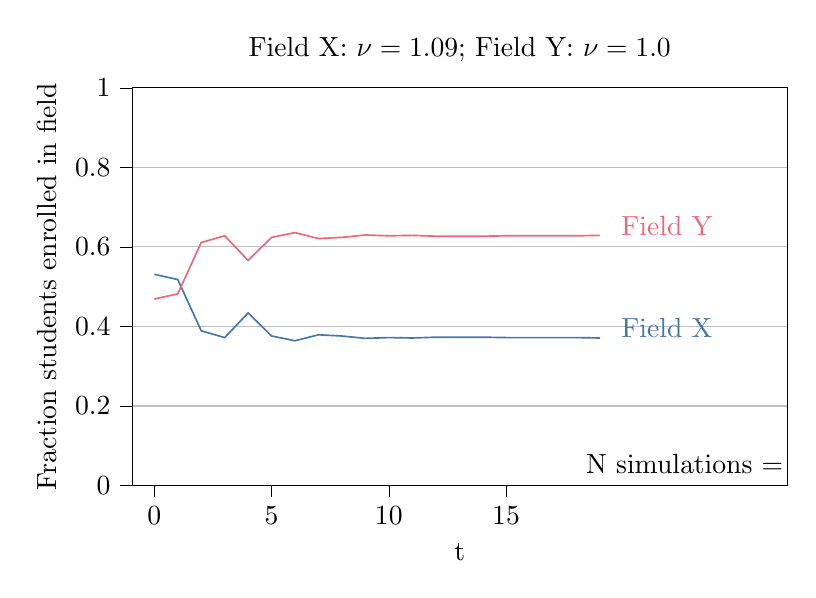
\begin{tikzpicture}

\definecolor{color0}{rgb}{0.266666666666667,0.466666666666667,0.666666666666667}
\definecolor{color1}{rgb}{0.933333333333333,0.4,0.466666666666667}

\begin{axis}[
height=6.6314113761540705cm,
tick align=outside,
tick pos=left,
title={Field X: \(\displaystyle \nu=1.09\); Field Y: \(\displaystyle \nu=1.0\)},
width=9.904475999999999cm,
x grid style={white!69.0196078431373!black},
xlabel={t},
xmin=-0.95, xmax=27,
xtick style={color=black},
xtick={0,5,10,15},
xticklabels={\(\displaystyle 0\),\(\displaystyle 5\),\(\displaystyle 10\),\(\displaystyle 15\)},
ylabel={Fraction students enrolled in field},
ymajorgrids,
ymin=0, ymax=1,
ytick style={color=black},
ytick={0,0.2,0.4,0.6,0.8,1},
yticklabels={\(\displaystyle 0\),\(\displaystyle 0.2\),\(\displaystyle 0.4\),\(\displaystyle 0.6\),\(\displaystyle 0.8\),\(\displaystyle 1\)}
]
\addplot [semithick, color0]
table {%
0 0.531000018119812
1 0.51800000667572
2 0.388999938964844
3 0.371999979019165
4 0.434000015258789
5 0.375999927520752
6 0.363999962806702
7 0.378999948501587
8 0.375999927520752
9 0.370000004768372
10 0.371999979019165
11 0.371000051498413
12 0.373000025749207
14 0.373000025749207
15 0.371999979019165
18 0.371999979019165
19 0.371000051498413
};
\addplot [semithick, color1]
table {%
0 0.468999981880188
1 0.48199999332428
2 0.611000061035156
3 0.628000020980835
4 0.565999984741211
5 0.624000072479248
6 0.635999917984009
7 0.621000051498413
8 0.624000072479248
9 0.629999995231628
10 0.628000020980835
11 0.628999948501587
12 0.626999974250793
14 0.626999974250793
15 0.628000020980835
18 0.628000020980835
19 0.628999948501587
};
\draw (axis cs:19.5,0.371) node[
  anchor=base west,
  text=color0,
  rotate=0.0
]{Field X};
\draw (axis cs:19.5,0.629) node[
  anchor=base west,
  text=color1,
  rotate=0.0
]{Field Y};
\draw (axis cs:18,0.03) node[
  anchor=base west,
  text=black,
  rotate=0.0
]{N simulations = 1000};
\end{axis}

\end{tikzpicture}

\end{figure}
\hyperlink{app_v_effects}{\beamerbutton{$\nu$ effects}}
\hyperlink{sim_beliefs}{\beamerbutton{Return: belief simulation}}

\end{frame}


%%%%%%%%%%%%%%%%%%%%%%%%%%%%%%%%%%%%%%%%%%%%%%%%%%%%%%%%%%%%%%%%%%%%%%%%%%%%%%%%
\begin{frame}{$\nu$ effects}\label{app_v_effects}

\begin{figure}
\centering
% This file was created by tikzplotlib v0.9.2.
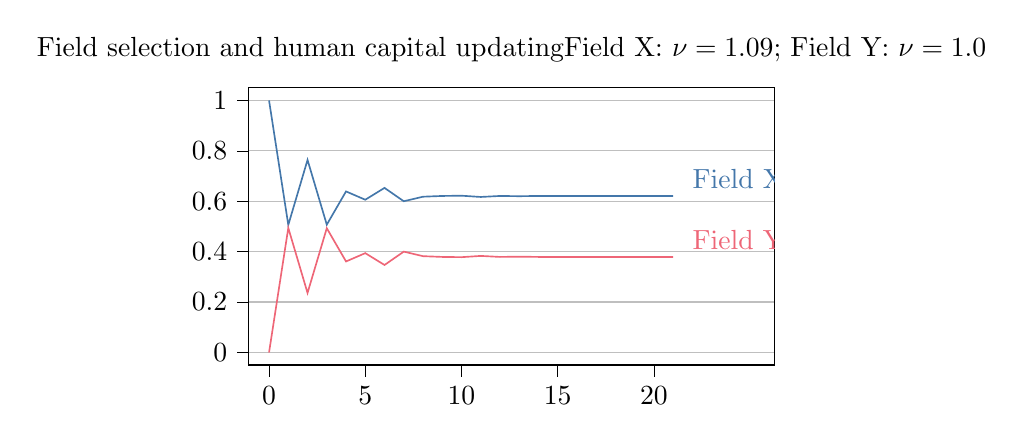
\begin{tikzpicture}

\definecolor{color0}{rgb}{0.266666666666667,0.466666666666667,0.666666666666667}
\definecolor{color1}{rgb}{0.933333333333333,0.4,0.466666666666667}

\begin{axis}[
height=5.101085673964669cm,
tick align=outside,
tick pos=left,
title={Field selection and human capital updating \\ Field X: \(\displaystyle \nu=1.09\); Field Y: \(\displaystyle \nu=1.0\)},
width=8.25373cm,
x grid style={white!69.0196078431373!black},
xmin=-1.05, xmax=26.25,
xtick style={color=black},
xtick={0,5,10,15,20},
xticklabels={\(\displaystyle 0\),\(\displaystyle 5\),\(\displaystyle 10\),\(\displaystyle 15\),\(\displaystyle 20\)},
ymajorgrids,
ymin=-0.05, ymax=1.05,
ytick style={color=black},
ytick={0,0.2,0.4,0.6,0.8,1},
yticklabels={\(\displaystyle 0\),\(\displaystyle 0.2\),\(\displaystyle 0.4\),\(\displaystyle 0.6\),\(\displaystyle 0.8\),\(\displaystyle 1\)}
]
\addplot [semithick, color0]
table {%
0 1
1 0.506
2 0.764
3 0.507
4 0.639
5 0.606
6 0.653
7 0.6
8 0.618
9 0.621
10 0.622
11 0.617
12 0.621
13 0.62
14 0.621
15 0.621
16 0.621
17 0.621
18 0.621
19 0.621
20 0.621
21 0.621
};
\addplot [semithick, color1]
table {%
0 0
1 0.494
2 0.236
3 0.493
4 0.361
5 0.394
6 0.347
7 0.4
8 0.382
9 0.379
10 0.378
11 0.383
12 0.379
13 0.38
14 0.379
15 0.379
16 0.379
17 0.379
18 0.379
19 0.379
20 0.379
21 0.379
};
\draw (axis cs:21.5,0.651) node[
  anchor=base west,
  text=color0,
  rotate=0.0
]{Field X};
\draw (axis cs:21.5,0.409) node[
  anchor=base west,
  text=color1,
  rotate=0.0
]{Field Y};
\end{axis}

\end{tikzpicture}

\end{figure}
\hyperlink{app_ability_v_effect}{\beamerbutton{Return: $\alpha_{X0} \nu_X = \alpha_{Y0} \nu_Y$}}
\hyperlink{sim_beliefs}{\beamerbutton{Return: belief simulation}}
\hyperlink{sim_ability}{\beamerbutton{Return: ability simulation}}

\end{frame}
